% Simpson-type formula for the integral of M(x) m(x)
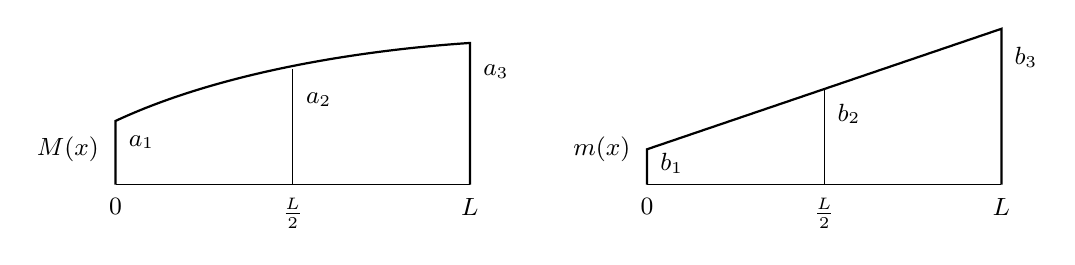
\begin{tikzpicture}[scale=0.9,font=\small]
  \begin{scope}
    \draw (0,0) -- (5,0);
    \draw[thick] (0,0) -- (0,0.9) .. controls (1.5,1.6) and (3.5,1.9) .. (5,2.0) -- (5,0);
    \draw (2.5,0) -- (2.5,1.63);
    \node[right] at (0.05,0.6) {$a_1$}; \node[right] at (2.55,1.2) {$a_2$}; \node[right] at (5.05,1.6) {$a_3$};
    \node[left] at (-0.1,0.5) {$M(x)$};
    \node[below] at (0,-0.05) {0}; \node[below] at (2.5,-0.05) {$\frac L2$}; \node[below] at (5,-0.05) {$L$};
  \end{scope}
  \begin{scope}[xshift=7.5cm]
    \draw (0,0) -- (5,0);
    \draw[thick] (0,0) -- (0,0.5) -- (5,2.2) -- (5,0);
    \draw (2.5,0) -- (2.5,1.35);
    \node[right] at (0.05,0.3) {$b_1$}; \node[right] at (2.55,1.0) {$b_2$}; \node[right] at (5.05,1.8) {$b_3$};
    \node[left] at (-0.1,0.5) {$m(x)$};
    \node[below] at (0,-0.05) {0}; \node[below] at (2.5,-0.05) {$\frac L2$}; \node[below] at (5,-0.05) {$L$};
  \end{scope}
\end{tikzpicture}
